\documentclass[10pt, conference, compsocconf]{IEEEtran}
%\usepackage[dvipdfmx]{color}
%\usepackage[dvipdfmx]{graphicx}
\usepackage{epsfig}
\usepackage[tight,footnotesize]{subfigure}
\usepackage{subfigure}
\usepackage{url}
\usepackage{cite}
\usepackage{comment}
\usepackage{listings}

%-----------------------------------------
% need for camera-ready
%\pagestyle{empty}
%----------------------------------------

\begin{document}

\title{GPU Implementations of Object Detection using HOG
Features and Deformable Models}

\author{
\IEEEauthorblockN{Manato Hirabayashi, Shinpei Kato, Masato Edahiro, and
Kazuya Takeda}
\IEEEauthorblockA{School of Information Science\\Nagoya University}
\and
\IEEEauthorblockN{Taiki Kawano and Seiichi Mita}
\IEEEauthorblockA{Research Center for Smart Vehicles\\Toyota
Technological Institute}
}


\maketitle

%%%%%%%%%%%%%%%%%%%%%%%%%%%%%%%%%%%
%% listings setting
\lstset{%
  language={C},
  basicstyle={\small},%
  identifierstyle={\small},%
  commentstyle={\small\itshape},%
  keywordstyle={\small\bfseries},%
  ndkeywordstyle={\small},%
  stringstyle={\small\itshape},
  frame={single},
  breaklines=true,
  columns=[l]{fullflexible},%
  numbers=left,%
  xrightmargin=5pt,%
  xleftmargin=10pt,%
  numberstyle={\scriptsize},%
  stepnumber=1,
  numbersep=5pt,%
  lineskip=-0.5ex,%
  showspaces=false
}
%%%%%%%%%%%%%%%%%%%%%%%%%%%%%%%%%%%

%-----------------------------------------
% need for camera-ready
%\thispagestyle{empty}

Visione-based object detection using camera sensors is an essential piece
of perception for autonomous vehicles.
Various combinations of features and models can be applied to increase
the quality and speed of object detection.
A well-known approach uses histograms of oriented gradients (HOG)
with deformable models to detect a car in an image.
A major challenge of this approach can be found in computational cost
introducing a real-time constraint problem in the real world.
In this paper, we present implementation techniques using graphics
processing units (GPUs) to accelerate computations of similarity scores
of the input image and the pre-defined models.
Our implementation considers not only the algorithm part but also the
entire program structure.
We experimentally show that our implementation using commodity GPUs can
achieve speedups of 1.5x to 3x in frame-rate over sequential and
multithreaded implementations using traditional CPUs.

\begin{IEEEkeywords}
 GPGPU; Computer Vision; Object Detection
\end{IEEEkeywords}

\section{Introduction}
\label{sec:introduction}

Grand challenges of cyber-physical systems (CPS) include a high
computational cost of understanding the physical world.
Image-based object detection is one of compute-intensive tasks for CPS.
For example, an autonomous vehicle needs to detect and track other
vehicles by itself.
Current autonomous driving technologies \cite{Guizzo11, Levinson11,
Urmson08} tend to rely on active sensors such as GPS, RADAR, and LIDAR
\cite{Kirchner00, Streller02} together with very accurate pre-configured
maps, but the use of passive camera sensors is becoming more practical
due to recent advances in computer vision \cite{Dalal05, Felzenszwalb05,
Felzenszwalb10}: vision-based object detection can be applied for
various ranges and orientations.
In particular, histograms of oriented gradients (HOG) \cite{Dalal05}
features provide reliable high-level representations of an image
underlying many state-of-the-art object detection
algorithms~\cite{Felzenszwalb10, Geiger12, Rybski10, Suard06, Zhu06}.
However, a major concern of HOG-based object detection remains in
computational cost.

Previous work on the implementation of HOG-based object detection are
limited to either hardware implementations \cite{Kadota09, Karakaya09,
Komorkiewicz12} or specific parts of the HOG algorithm \cite{Chen11,
Prisacariu09}.

\section{Assumption}
\label{sec:assumption}

We consider the system composed of a multicore CPU and commodity GPU.
They communicate with each other via the PCIe bus.
We use CUDA \cite{NVIDIA_CUDA} for GPU programming, whose development
environment can be downloaded from NVIDIA's website \cite{NVIDIA_NVCC}.
Input images are loaded from pre-captured JPEG files, since we focus on
a high computational cost of image processing.
Systemized coordinations of computations and I/O devices are outside the
scope of this paper.
The use of multiple GPUs is also not in consideration.

We follow the object detection method presented by Felzenszwalb
\textit{et. al.} \cite{Felzenszwalb10}, where objects are represented by
HOG features \cite{Dalal05} and the detectors is composed of a ``root''
filter plus a set of ``parts'' filters that allow visual appearance to
be modeled at multiple scales.
This is one of the most recognized approach to object detection.
See \cite{Felzenszwalb10} for the detail.

\begin{figure}[t]
 \begin{center}
  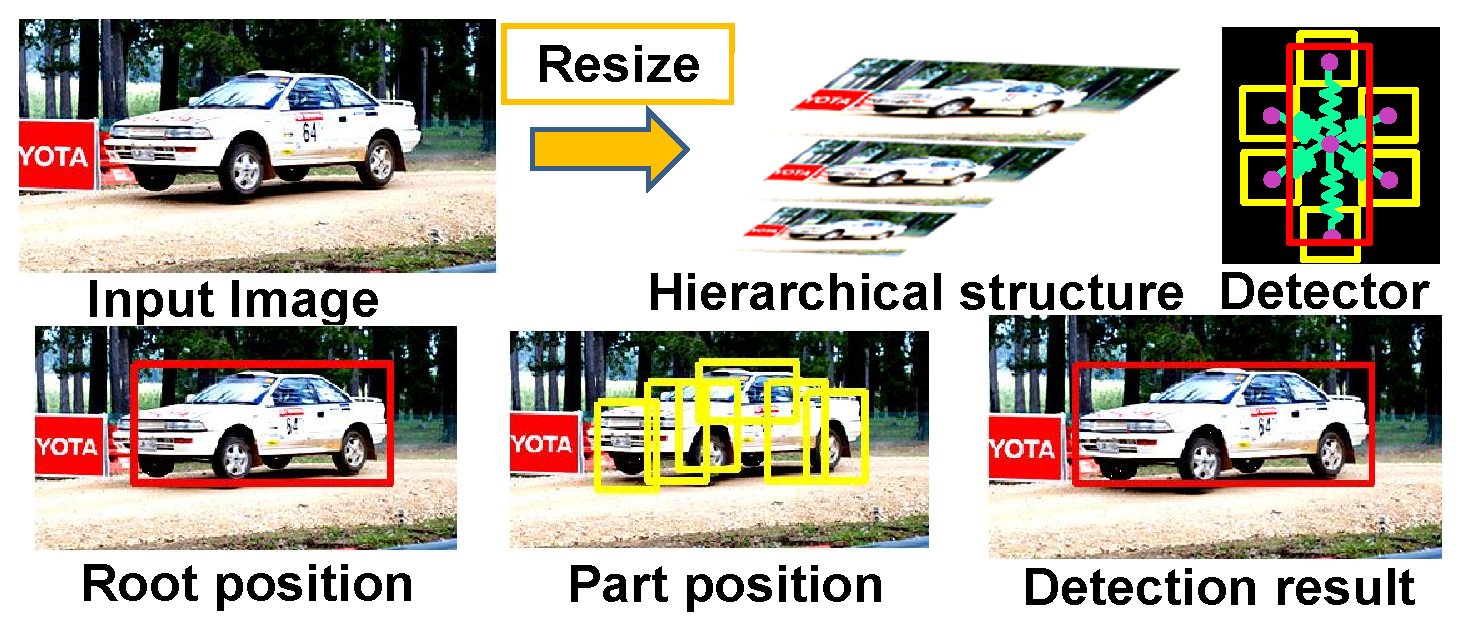
\includegraphics[width=\hsize]{fig/deformable_model.eps}\\
  \caption{Vehicle detection flow with deformable models.}
  \label{fig:deformable_model}
 \end{center}
\end{figure}

Object detection often requires a machine learning phase to construct
the object models.
We assume that this learning phase has already been done a priori and
the object models are stored in the system.
Particularly we restrict our attention to vehicle detection in this
paper, utilizing the vehicle models provided by prior work
\cite{Niknejad12}.
A brief concept of this approach is illustrated in
Fig.~\ref{fig:deformable_model}.
Although these models achieve a high detection rate, the computational
cost of scoring similarity of an imput image and the models using HOG
features is very expensive.
Specifically they include $2$ root filters and $12$ part filters, each
of which needs to be scored against $32$ resized images.
The scoring could be conducted for every squire of a few pixels
independently.
In consequence, there are approximately 10 million computational
blocks for a single high-definition image, while the frame-rate needs to
meet 10$\sim$20 frames per second (FPS) for practical use.
This data-parallel compute-intensive nature of HOG-based object
detection motivates the use of GPUs in this paper.

The CPU implementation of HOG-based vehicle detection has already been
developed in prior work \cite{Niknejad12}.
It leverages the POSIX \textit{pthread} to parallelize the scoring per
filter on a multicore CPU.
While we use this multicore implementation for a performance comparison
as it is, we also serialize it to execute on a single core so that we
can compare our GPU implementation to two variants of the CPU
implementation.

\section{GPU Implementation}
\label{sec:implementation}

This paper presents GPU implementations of the existing object
detection program using a popular computer vision technique
\cite{Niknejad12}.
Our contribution is distinguished from prior GPU implementations work
\cite{Chen11, Prisacariu09} in that we analyze the performance
characteristics of the object detection program to figure out what part
of the program should be accelerated using the GPU and our
implementations build on this analysis optimizing performance.

Note that this paper focuses on vehicle detection but the presented GPU
implementations and our technical contribution can be applied for other
object detection methods using HOG features and deformable models.

\subsection{Basic Understanding}
\label{sec:understanding}

In GPU programming, the GPU code and the input data typically need to be
copied from the host to the device memory before we launch a function,
\textit{a.k.a.}, a compute kernel, on the GPU.
The output data also needs to be copied back from the device to the host
memory so that the CPU can read them.
Hence the GPU-accelerated computation comes at the expense of the
offloading overhead.
Another shortcoming of the GPU is its relatively low operating frequency
as compared to the CPU due to the presence of a significant number of
compute cores.
These trade-offs must be addressed to benefit from GPU programming; it
is a complex undertaking for programmers to ascertain appropriate
computational blocks that can accelerate on the GPU.
Nonetheless this massively parallel computing architecture is becoming a
trend in the state of the art.
Given that GPUs outperform traditional multithreaded and multicore CPUs
in peak performance by an order of magnitude \cite{Kato13_2}, it is
worth exploring a more efficient way of GPU programming.
This paper provides a guideline of how to use GPUs in an efficient way
for vision-based object detection.

\subsection{Program Analysis}
\label{sec:analysis}

As aforementioned, the usage of the GPU depends highly on the program
structure.
If the program does not contain data-parallel compute-intensive blocks,
the GPU is not effective at all.
Therefore it is important to analyze the program prior to coding and
implementation.
The following is a summary of the program sequence for HOG-based object
detection using the deformable models.
The detailed procedure and algorithm description are presented in
\cite{Felzenszwalb10, Niknejad12}.

\begin{enumerate}
\item Load an input image.
\item Load the pre-defined object models.
\item Calculate HOG features for all resized variants of the input
      image, often referred to as a \textit{HOG pyramid}.
\item Calculate similarity scores for every set of the root/part filters
      and the resized HOG images.
\item Detect an object region based on a summation of the similarity
      scores.
\item Recognize an object based on the detection result.
\item Output the recognition result.
\end{enumerate}

\begin{figure}[t]
 \begin{center}
  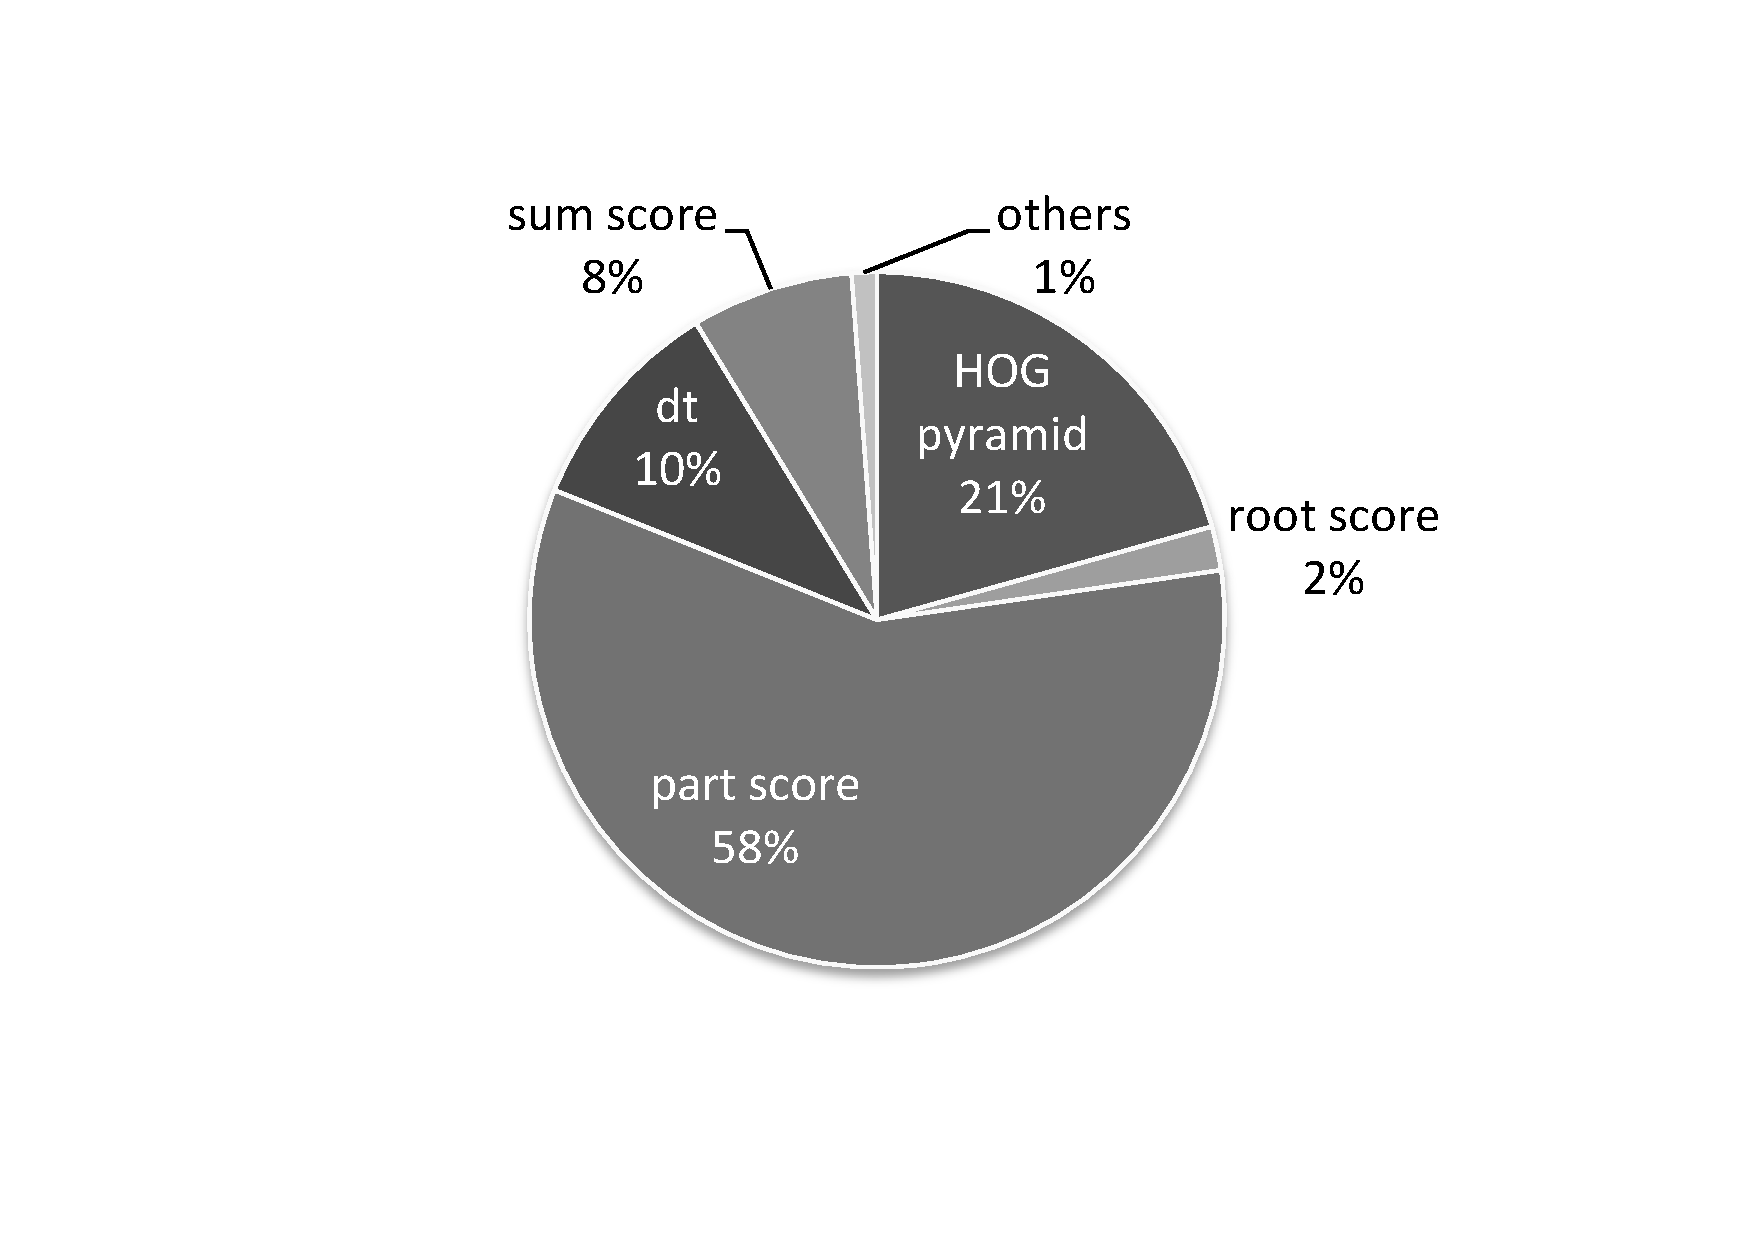
\includegraphics[width=\hsize]{fig/breakdown.pdf}\\
  \caption{The breakdown of computation times.}
  \label{fig:breakdown}
 \end{center}
\end{figure}

In order to identify computationally time-consuming blocks of the object
detection program, we conducted a preliminary measurement running the
original sequential code \cite{Niknejad12} on a generic Intel Core i7
2700K CPU.
The measurement method is straightforward.
We find high-level \textit{for} loops (in case that the program is
written in the C-like language) by scanning the program structure and
make a timestamp for each loop.
The result of measurement is shown in Fig.~\ref{fig:breakdown}.
Note that a label ``others'' represents the computation time excluding
the high-level \textit{for} loops.
This breakdown of computation times provides us with a hint of how to
approach GPU implementations.
Specifically an obvious computational bottleneck appears in the
calculation of similarity scores against the part filters, which
corresponds to partly ``Step 4)`` in the above program sequence.
This block dominates $58\%$ of the total time.
On the other hand, the calculation of HOG features corresponding ``Step
3)'' spends $21\%$ of the total time, while the detection and recognition
of the object, \textit{i.e.}, ``Step 5)'' and ``Step 6)'', contribute to
$10\%$ and $8\%$ of the total time respectively.

Our analysis conducted herein implies that even a simple time
measurement highlighting only the program structure without awareness of
the program context is helpful enough to understand computational
bottlenecks of the program.
In our case, it turned out that the most portion of the total time is
spent in the \textit{for} loops, which means that this program contains
a very high degree of parallelism and could be accelerated on the GPU.

\subsection{Implementation Approach}

We parallelize all the high-level \textit{for} loops of the program
using the GPU.
According to the measurement result in Fig.~\ref{fig:breakdown}, the
scoring of the root filters is a minor factor ($2\%$) of the total
time, but its program structure is almost identical to that of the part
filters and they adhere to continuous blocks.
Hence we include it to the GPU code.
In the rest of this section, we focus on the implementation of the
scoring of these filters, which is the most dominant part of the
program, due to a space constraint.

\begin{figure}[t]
 \begin{center}
  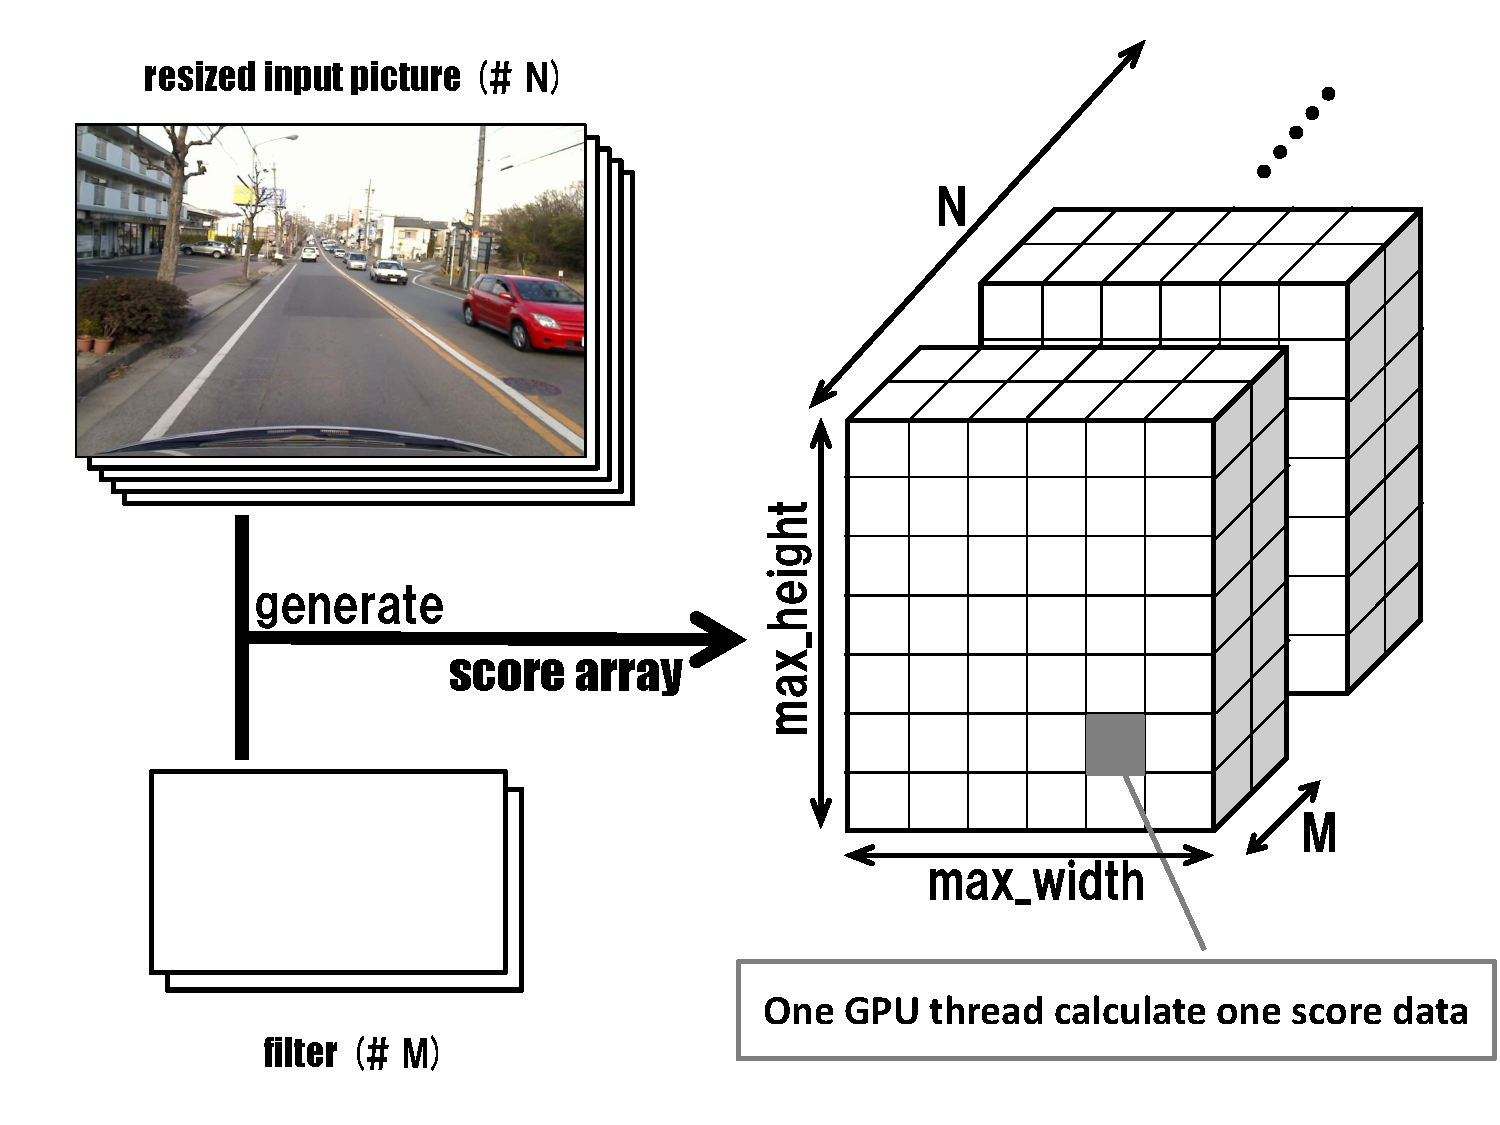
\includegraphics[width=\hsize]{fig/threads_shape.pdf}\\
  \caption{The number of compute threads and their block shape.}
  \label{fig:threads_shape}
 \end{center}
\end{figure}

Fig.~\ref{fig:threads_shape} illustrates a conceptual structure and flow
of our GPU implementation.
We have 32 resized pictures to be able to detect different sizes of the
object, \textit{i.e.}, \texttt{N} is 32.
We also have $2$ root filters and $12$ part filters to be able to detect
different shapes or angles of the object, \textit{i.e.}, \texttt{M} is 2
or 12.
A minimum piece of the similarity score for a HOG representation and an
object model can be calculated for each pixel of the filtered area
independently.
This area could be larger than a squire of $100$ pixels (equivalent to
\texttt{max\_width} $\times$ \texttt{max\_height}) for a $640 \times 480$
size of an image when using the trained data obtained from previous work
\cite{Niknejad12}.
Therefore the number of producible compute threads could be an order of
millions in this setup.
We shape these threads by blocks and grids for CUDA as shown in
Fig.~\ref{fig:threads_shape} where each block size is \texttt{max\_width}
$\times$ \texttt{max\_height} $\times$ \texttt{M} and each grid size is
\texttt{N}.
This shape is considered for ease of programming and a different shape
may further improve performance but such a fine-grained performance
tuning is outside the scope of this paper.

\subsection{GPU Programming}
\section{Evaluation}
\label{sec:evaluation}

This section demonstrates performance improvements brought by our GPU
implementations for the existing vehicle detection program
\cite{Niknejad12}.
We also discuss the details of performance comparisons among our GPU
implementations and traditional CPU implementations identifying the
fundamental factors that allow GPUs to outperform CPUs.

\subsection{Experimental Setup}
\label{sec:setup}

We prepare three variants of the vehicle detection program implemented
using (i) a single CPU core, (ii) multiple CPU cores, (iii) and
massively parallel GPU compute cores.
The CPU implementations use the Intel Core i7 3930K (@3.2GHz) and the
Xeon E5-2643 (@3.3GHz) series while we provide several different GPUs
for the GPU implementations: namely NVIDIA GeForce GTX 560 Ti, GTX 580,
GTX 680, GTX TITAN, and Tesla K20Xm.
The same set of 10 images as previous work \cite{Niknejad12} is used as
input data and their average execution time is considered as major
performance metrics.
Note that this execution time includes all relevant pieces of image
processing such as image loading and output rendering in addition to the
primary object detection block.

\subsection{Experimental Results}
\label{sec:results}

\begin{figure}[t]
 \begin{center}
  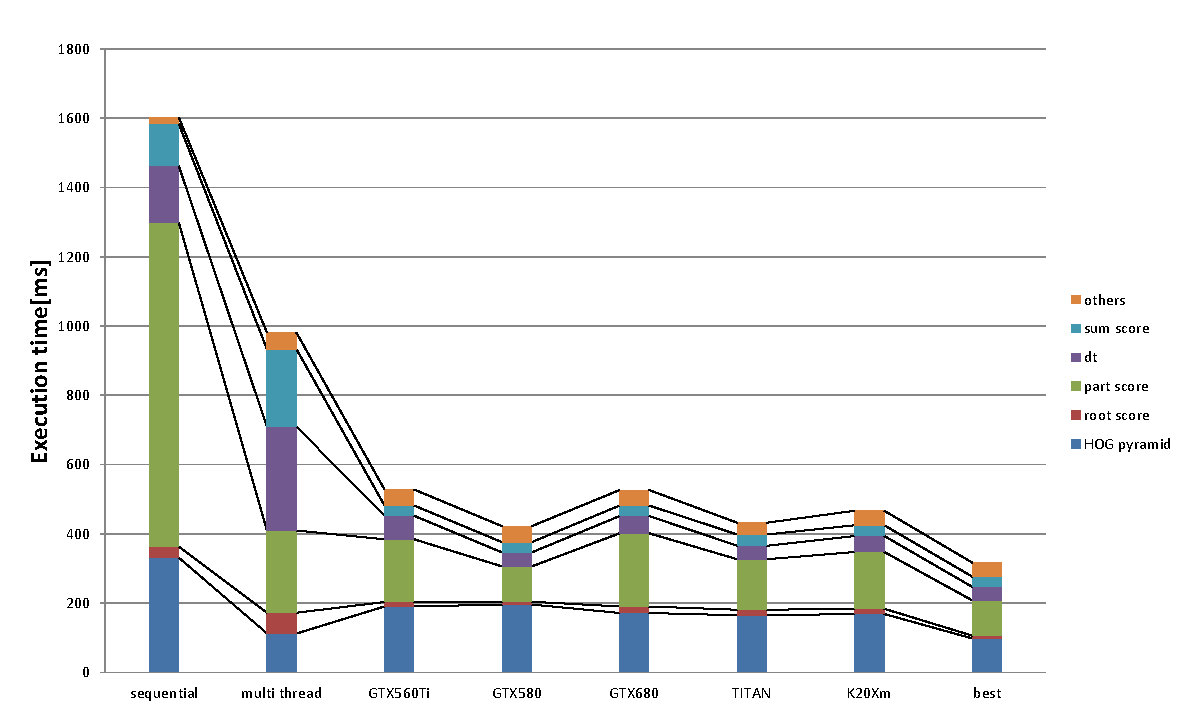
\includegraphics[width=\hsize]{fig/float_exe_time.eps}\\
  \caption{Execution times of the single-precision floating-point program.}
  \label{fig:float_exe_time}
 \end{center}
\end{figure}

\begin{figure}[t]
 \begin{center}
  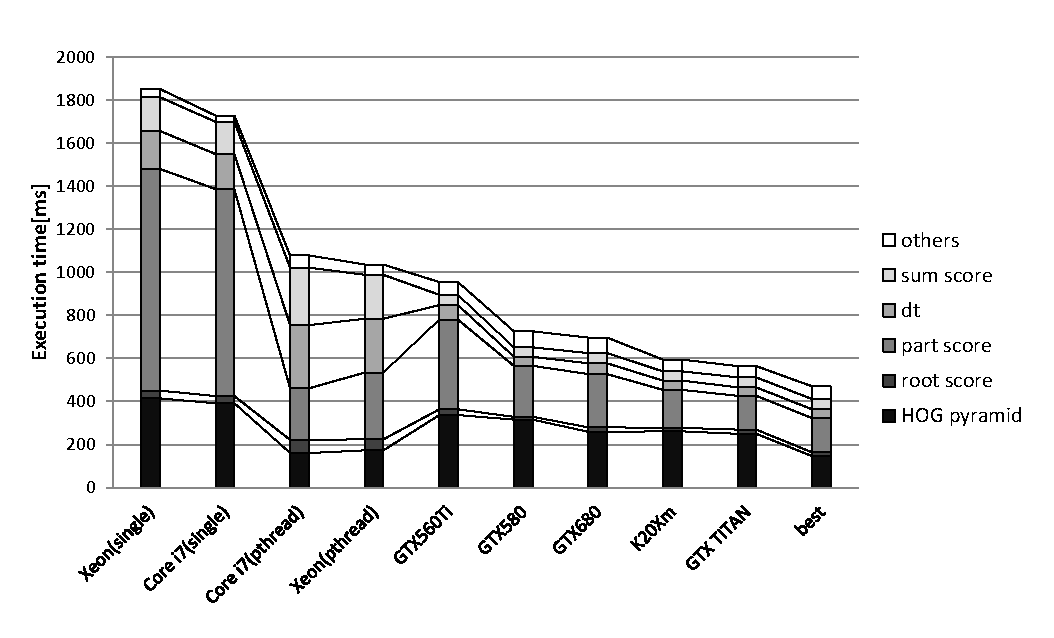
\includegraphics[width=\hsize]{fig/double_exe_time.eps}\\
  \caption{Execution times of the double-precision floating-point program.}
  \label{fig:double_exe_time}
 \end{center}
\end{figure}

Fig.~\ref{fig:float_exe_time} shows the execution times of all variants
of the vehicle detection program configured to use single-precision
floating-point operations.
The dimensions of input images are 640$\times$480 pixels.
``XXX(single)'' uses a single CPU core for the corresponding CPU series
while ``XXX(multicore)'' uses multiple CPU cores with \textit{pthread}.
Other labels except for ``best'' represent our GPU implementations using
the corresponding GPUs; ``best'' describes the best combination of the
GPU and CPU implementations.
For the GPU implementations, we shape each CUDA block by $8 \times 8$
threads.
It is notable to see that most computational blocks benefit from GPUs
but only the HOG calculation prefers the multicore implementation.
This is attributed to the fact that the HOG calculation contains atomic
operations as illustrated in Listing~\ref{lst:hog} that could squeeze
massively parallel threads of the GPU.

Comparisons among the GPUs as well as those among the CPUs provide an
intriguing observation.
The GPUs based on the state-of-the-art \textit{Kepler}
architecture \cite{NVIDIA_Kepler} are inferior to those based on the
old \textit{Fermi} architecture \cite{NVIDIA_Fermi}.
Albeit a significant number of compute cores with the enhanced
multithreading mechanism, the Kepler GPUs operate at lower frequency
than the Fermi GPUs due to their complex architecture.
Since the vehicle detection program employs a lot of compute-intensive
blocks as depicted through Listing~\ref{lst:score} to \ref{lst:hog}, the
operating  frequency is more dominating than the architectural benefit.
This is a useful finding toward the future development of GPU-based
image processing.
It is also remarkable that the Core i7 CPU is slightly faster than the
Xeon CPU.
Since the experiment is limited to a single process, we suspect that a
desktop-oriented design of the Core i7 CPU is preferred to a
server-oriented design of the Xeon CPU.

As a whole, the best performance is obtained from such a setup that
uses the multicore implementation for the HOG calculation while
offloading other computational blocks to the GeForce GTX 580 GPU.
It results in a speed-up of more than 3x to 5x for the execution of
vehicle detection over the traditional single-core CPU implementation
and the multicore CPU implementation respectively.
This scale of speed-up for the overall execution of a complex real-world
application is a significant contribution, whereas an order-of-magnitude
speed-up has been reported for particular blocks of the program and the
algorithm in previous work \cite{Chen11, Prisacariu09}.
Our results truly demonstrate the current performance status of
state-of-the-art GPUs for practical vehicle detection.

Fig. \ref{fig:double_exe_time} shows the execution times of all variants
of the vehicle detection problem configuired to use double-precision
floating-point operations.
Unlike the single-precision scenario, the Kepler GPUs outperform the
Fermi GPUs.
This explains that the double-precision performance of GPUs is improved
as the generation of GPUs advances.
Another notable finding is that the TITAN GPU is slightly faster than
the K20Xm GPU for our vehicle detection program.
This is due to a slightly higher operating frequency of the TITAN GPU.
Since the TITAN GPU is a consumer market price while the K20Xm is a very
expensive supercomputing device, we suggest that the vehicle detection
program uses the TITAN GPU for a better cost performance.

Henceforth we restrict our attention to the single-precision
floating-point version of the vehicle detection program.
Note that similar performance characteristics were also observed in the
double-precision version through our experiments but they are omitted
herein due to a space constraint.

\begin{figure}[t]
 \begin{center}
  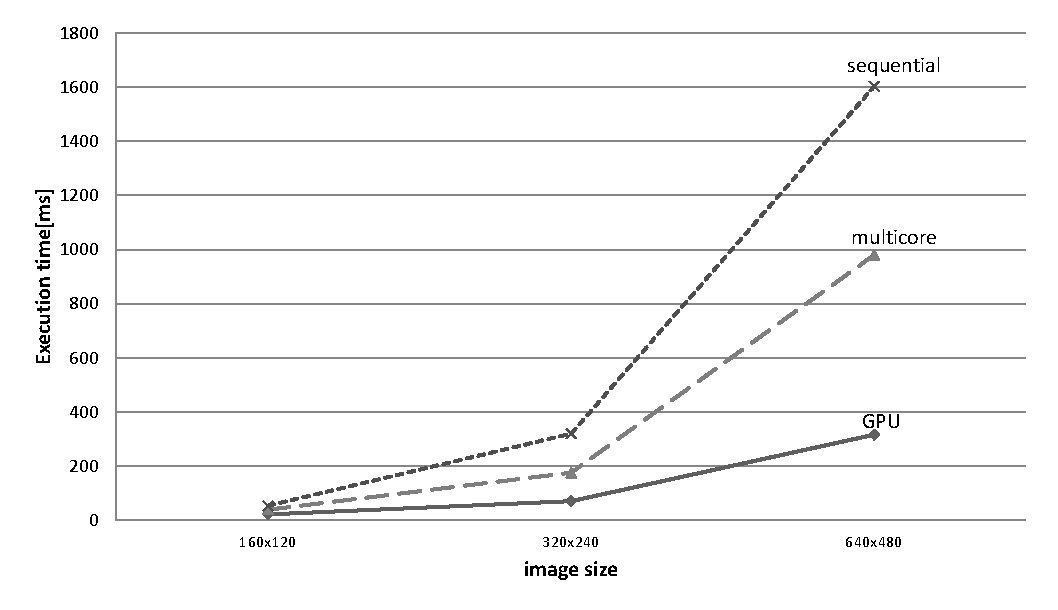
\includegraphics[width=\hsize]{fig/time_on_image_size.eps}\\
  \caption{Impact of the image size on execution times.}
  \label{fig:time_on_image_size}
 \end{center}
\end{figure}

Fig. \ref{fig:time_on_image_size} shows the impact of the image size on
execution times. 
The GPU implementation uses the GeForce GTX 580 GPU, which is the best
performer in all the GPUs demonstrated in Fig. \ref{fig:float_exe_time}.
The lessons learned from this experiment are that the execution time of
the vehicle detection program is proportionally influenced by the input
image size.
Therefore the benefit of our GPU implementations as compared to the
traditional CPU implementations would hold for more high-resolution
image processing.

\begin{figure}[t]
 \begin{center}
  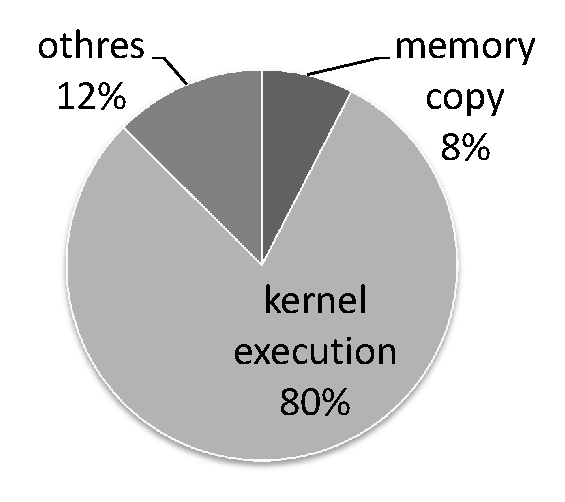
\includegraphics[width=0.5\hsize]{fig/breakdown_gpu.eps}\\
  \caption{The breakdown of execution times of the GPU implementation.}
  \label{fig:breakdown_gpu}
 \end{center}
\end{figure}

Fig. \ref{fig:breakdown_gpu} shows the breakdown of execution times of
the GPU implementation that achieves the best performance for the
vehicle detection program.
The memory copy overhead is often claimed to be a bottleneck in GPU
programming \cite{Jablin_PLDI11}, but our analysis explains that it is
not the case for the exhibited workload.
This means that further advances of GPU technology will lead to faster
implementations of the vehicle detection program, which encourages
future work to use state-of-the-art GPUs.

\begin{figure}[t]
 \begin{center}
  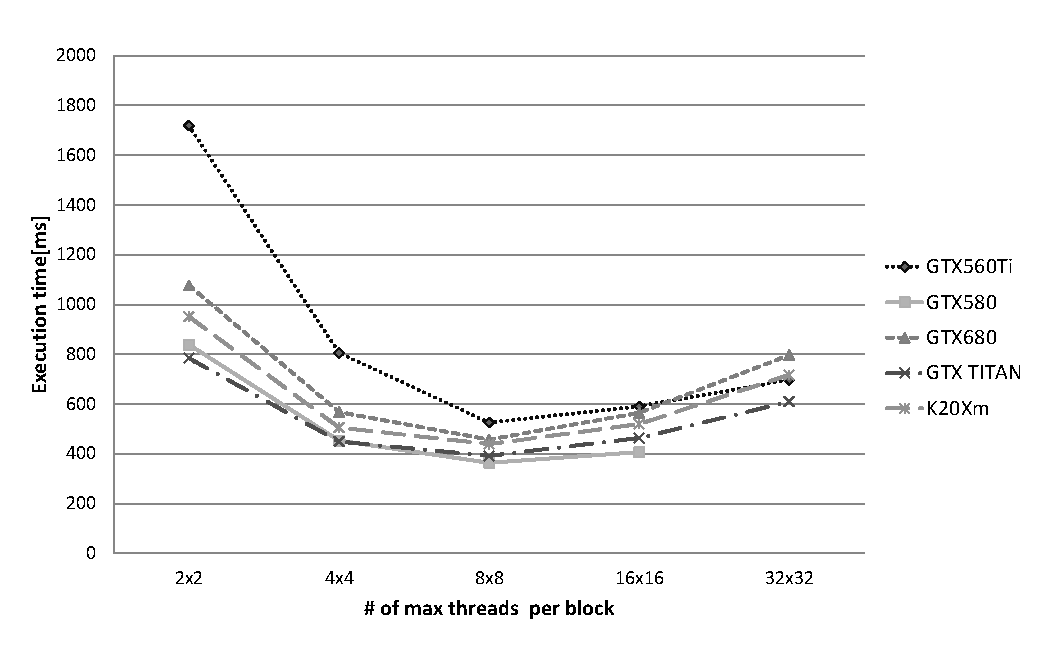
\includegraphics[width=\hsize]{fig/impact_of_blockshape.eps}\\
  \caption{Impact of the block shape on execution times.}
  \label{fig:impact_of_blockshape}
 \end{center}
\end{figure}

Fig. \ref{fig:impact_of_blockshape} shows the impact of the block shape
of GPU code on the execution times of the single-precision
floating-point vehicle detection program.
Particularly the number of threads in each block is varied to see how
the performance is affected.
Note that the Fermi GPUs cannot support 32$\times$32 threads per block
due to the hardware limitation.
From what we observed in our experiment, a configuration of 8$\times$8
threads exhibits the best performance for all the GPUs.
This is somewhat an intuitive expectation because each warp of the GPU
can contain up to 32 threads and a set of two warps is executed every
two cycles according to the NVIDIA GPU architecture.
Having less threads per block looses parallelism while introducing more
threads could cause resource confliction within a block.
Therefore a more in-depth investigation is required to truly optimize
performance.

\section{Conclusion}
\label{sec:conclusion}

In this paper, we have presented GPU implementations of HOG-based object
detection and their detailed performance evaluation.
Unlike preceding work that highly stressed on performance improvements,
our implementations are based on an analysis of performance bottlenecks
posed due to an introduction of the deformable models in HOG-based
object detection.
This approach ensures that the GPU truly accelerates appropriate
computational blocks.
Our experimental results using commodity GPUs showed that our GPU
implementations can speed up the existing HOG-based vehicle detection
program tailored to the deformable models by 3x to 5x over traditional
CPU implementations.
Given that this performance improvement is obtained from the entire
program runtime rather than particular algorithm parts of the program,
our contribution is useful and significant for real-world applications
of vision-based object detection. 

To the best of our knowledge, this is the first piece of work that made
a \textit{tight} coordination of object detection and parallel computing
-- a core challenge of CPS.
Specifically we showed that a measured and structured way of GPU
programming is efficient for the object detection program and quantified
the impact of GPUs in performance.
Our conclusion is that GPUs are promising to meet the required
performance of vision-based object detection in the real world.

In future work, we plan to complement this work with systematized
coordination of computations and I/O devices.
Since real-world applications require camera sensors to obtain input
images while GPUs are compute devices off the host computer, the data
I/O latency could become a non-trivial bottleneck on the data bus.
In this scenario, we need enhanced system support such as zero-copy
approaches \cite{Kato13} to minimize the data latency raised between
camera sensors and GPUs.
We also plan to augment our GPU implementations using multiple GPUs in
order to meet the real-time and real-fast requirement of real-world CPS
applications.


\bibliographystyle{plain}
{\footnotesize
\bibliography{references}
}

\end{document}



